\documentclass{tufte-handout}

\title{CS224n: Natural Language Processing with Deep Learning
       \thanks{Course Instructors: Christopher Manning, Richard Socher} \\
       \Large Lecture Notes: Part VI\thanks{Authors: Guillaume Genthial, Lucas Liu, Barak Oshri, Kushal Ranjan}}

\date{Winter 2017} % without \date command, current date is supplied

%\geometry{showframe} % display margins for debugging page layout

\usepackage{graphicx} % allow embedded images
  \setkeys{Gin}{width=\linewidth,totalheight=\textheight,keepaspectratio}
  \graphicspath{{notes6/}} % set of paths to search for images
\usepackage{amsmath}  % extended mathematics
\usepackage{amstext}  % extended text
\usepackage{booktabs} % book-quality tables
\usepackage{units}    % non-stacked fractions and better unit spacing
\usepackage{multicol} % multiple column layout facilities
\usepackage{lipsum}   % filler text
\usepackage{fancyvrb} % extended verbatim environments
\usepackage{placeins}
  \fvset{fontsize=\normalsize}% default font size for fancy-verbatim environments
\usepackage[normalem]{ulem}
\usepackage{algpseudocode}
\usepackage{algorithm}
\usepackage{color}


% tikz package
\usepackage{tikz}
\usetikzlibrary{patterns, shapes,calc,positioning,arrows,mindmap,matrix}
\usetikzlibrary{decorations.pathreplacing}

% Standardize command font styles and environments
\newcommand{\doccmd}[1]{\texttt{\textbackslash#1}}% command name -- adds backslash automatically
\newcommand{\docopt}[1]{\ensuremath{\langle}\textrm{\textit{#1}}\ensuremath{\rangle}}% optional command argument
\newcommand{\docarg}[1]{\textrm{\textit{#1}}}% (required) command argument
\newcommand{\docenv}[1]{\textsf{#1}}% environment name
\newcommand{\docpkg}[1]{\texttt{#1}}% package name
\newcommand{\doccls}[1]{\texttt{#1}}% document class name
\newcommand{\docclsopt}[1]{\texttt{#1}}% document class option name
\newenvironment{docspec}{\begin{quote}\noindent}{\end{quote}}% command specification environment
\newcommand{\argmin}{\operatornamewithlimits{argmin}}
\newcommand{\argmax}{\operatornamewithlimits{argmax}}
\newcommand{\textunderscript}[1]{$_{\text{#1}}$}

\setcounter{secnumdepth}{3}

\begin{document}

\maketitle% this prints the handout title, author, and date


\textbf{Keyphrases: Seq2Seq and Attention Mechanisms, Neural Machine Translation, Speech Processing}
\section{Neural Machine Translation with Seq2Seq}
% from the Feb 16 lecture
So far in this class, we've dealt with problems of predicting a single output: an NER label for a word, the single most likely next word in a sentence given the past few, and so on. However, there's a whole class of NLP tasks that rely on \textit{sequential output}, or outputs that are sequences of potentially varying length. For example,
\begin{itemize}
\item \textbf{Translation:} taking a sentence in one language as input and outputting the same sentence in another language.
\item \textbf{Conversation:} taking a statement or question as input and responding to it.
\item \textbf{Summarization:} taking a large body of text as input and outputting a summary of it.
\end{itemize}
In these notes, we'll look at sequence-to-sequence models, a deep learning-based framework for handling these types of problems. This framework proved to be very effective, and has, in fewer than 3 years, become the standard for machine translation.

\subsection{Brief Note on Historical Approaches}
%At this point, it may help to consider how Seq2Seq is a departure from previous models.
In the past, translation systems were based on probabilistic models constructed from:
\begin{itemize}
\item a \textbf{translation model}, telling us what a sentence/phrase in a source language most likely translates into
\item a \textbf{language model}, telling us how likely a given sentence/phrase is overall.
\end{itemize}
These components were used to build translation systems based on words or phrases. As you might expect, a naive word-based system would completely fail to capture differences in ordering between languages (e.g. where negation words go, location of subject vs. verb in a sentence, etc).

Phrase-based systems were most common prior to Seq2Seq. A phrase-based translation system can consider inputs and outputs in terms of sequences of phrases and can handle more complex syntaxes than word-based systems. However, long-term dependencies are still difficult to capture in phrase-based systems.

The advantage that Seq2Seq brought to the table, especially with its use of LSTMs, is that modern translation systems can generate arbitrary output sequences after seeing the \textit{entire} input. They can even focus in on specific parts of the input automatically to help generate a useful translation.

\subsection{Sequence-to-sequence Basics}
Sequence-to-sequence, or "Seq2Seq", is a relatively new paradigm, with its first published usage in 2014 for English-French translation \footnote{Sutskever et al. 2014, "Sequence to Sequence Learning with Neural Networks"}. At a high level, a sequence-to-sequence model is an end-to-end model made up of two recurrent neural networks:
\begin{itemize}
\item an \textit{encoder}, which takes the model's input sequence as input and encodes it into a fixed-size "context vector", and
\item a \textit{decoder}, which uses the context vector from above as a "seed" from which to generate an output sequence.
\end{itemize}
For this reason, Seq2Seq models are often referred to as "encoder-decoder models." We'll look at the details of these two networks separately.


\subsection{Seq2Seq architecture - encoder}

The encoder network's job is to read the input sequence to our Seq2Seq model and generate a fixed-dimensional context vector $C$ for the sequence. To do so, the encoder will use a recurrent neural network cell -- usually an LSTM -- to read the input tokens one at a time. The final hidden state of the cell will then become $C$. However, because it's so difficult to compress an arbitrary-length sequence into a single fixed-size vector (especially for difficult tasks like translation), the encoder will usually consist of \textit{stacked} LSTMs: a series of LSTM "layers" where each layer's outputs are the input sequence to the next layer. The \textit{final} layer's LSTM hidden state will be used as $C$.

Seq2Seq encoders will often do something strange: they will process the input sequence \textit{in reverse}. This is actually done on purpose. The idea is that, by doing this, the \textit{last} thing that the encoder sees will (roughly) corresponds to the \textit{first} thing that the model outputs; this makes it easier for the decoder to "get started" on the output, which makes then gives the decoder an easier time generating a proper output sentence. In the context of translation, we're allowing the network to translate the first few words of the input as soon as it sees them; once it has the first few words translated correctly, it's much easier to go on to construct a correct sentence than it is to do so from scratch. See Fig. \ref{fig:basic_enc} for an example of what such an encoder network might look like.

\begin{marginfigure}
	\centering
	\includegraphics[width=\linewidth]{Encoder.png}
	\caption {Example of a Seq2Seq encoder network. This model may be used to translate the English sentence "what is your name?" Note that the input tokens are read in reverse. Note that the network is unrolled; each column is a timestep and each row is a single layer, so that horizontal arrows correspond to hidden states and vertical arrows are LSTM inputs/outputs.}
	\label{fig:basic_enc}
\end{marginfigure}

\subsection{Seq2Seq architecture - decoder}

The decoder is also an LSTM network, but its usage is a little more complex than the encoder network. Essentially, we'd like to use it as a language model that's "aware" of the words that it's generated so far \textit{and} of the input. To that end, we'll keep the "stacked" LSTM architecture from the encoder, but we'll initialize the hidden state of our first layer with the context vector from above; the decoder will literally use the context of the input to generate an output.

Once the decoder is set up with its context, we'll pass in a special token to signify the start of output generation; in literature, this is usually an <EOS> token appended to the end of the input (there's also one at the end of the output). Then, we'll run all three layers of LSTM, one after the other, following up with a softmax on the final layer's output to generate the first output word. Then, we \textit{pass that word into the first layer}, and repeat the generation. This is how we get the LSTMs to act like a language model. See Fig. \ref{fig:basic_dec} for an example of a decoder network.

Once we have the output sequence, we use the same learning strategy as usual. We define a loss, the cross entropy on the prediction sequence, and we minimize it with a gradient descent algorithm and back-propagation. Both the encoder and decoder are trained at the same time, so that they both learn the same context vector representation.

\subsection{Recap \& Basic NMT Example}
Note that there is no connection between the lengths of the input and output; any length input can be passed in and any length output can be generated. However, Seq2Seq models are known to lose effectiveness on very long inputs, a consequence of the practical limits of LSTMs.

To recap, let's think about what a Seq2Seq model does in order to translate the English "what is your name" into the French "comment t'appelles tu". First, we start with 4 one-hot vectors for the input. These inputs may or may not (for translation, they usually are) embedded into a dense vector representation. Then, a stacked LSTM network reads the sequence in reverse and \textit{encodes} it into a context vector. This context vector is a vector space representation of the notion of asking someone for their name. It's used to initialize the first layer of another stacked LSTM. We run one step of each layer of this network, perform softmax on the last layer's output, and use that to select our first output word. This word is fed back into the network as input, and the rest of the sentence "comment t'appelles tu" is \textit{decoded} in this fashion. During backpropagation, the encoder's LSTM weights are updated so that it learns a better vector space representation for sentences, while the decoder's LSTM weights are trained to allow it to generate grammatically correct sentences that are relevant to the context vector.
\begin{marginfigure}
	\centering
	\includegraphics[width=\linewidth]{Decoder.png}
	\caption {Example of a Seq2Seq decoder network. This decoder is decoding the context vector for "what is your name" (see Fig. \ref{fig:basic_enc} into its French translation, "comment t'appeles tu?" Note the special "GO" token used at the start of generation, and that generation is in the forward direction as opposed to the input which is read in reverse. Note also that the input and output do not need to be the same length.}
	\label{fig:basic_dec}
    $$ $$
\end{marginfigure}


\subsection{Bidirectional RNNs}
Recall from earlier in this class that dependencies in sentences don't just work in one direction; a word can have a dependency on another word before \textit{or} after it. The formulation of Seq2Seq that we've talked about so far doesn't account for that; at any timestep, we're only considering information (via the LSTM hidden state) from words \textit{before} the current word. For NMT, we need to be able to effectively encode any input, regardless of dependency directions within that input, so this won't cut it.

Bidirectional RNNs fix this problem by traversing a sequence in both directions and concatenating the resulting outputs (both cell outputs and final hidden states). For every RNN cell, we simply add another cell but feed inputs to it in the opposite direction; the output $o_t$ corresponding to the $t$'th word is the concatenated vector $\begin{bmatrix} o^{(f)}_t & o^{(b)}_t \end{bmatrix}$, where $o^{(f)}_t$ is the output of the forward-direction RNN on word $t$ and $o^{(b)}_t$ is the corresponding output from the reverse-direction RNN. Similarly, the final hidden state is $h = \begin{bmatrix} h^{(f)} & h^{(b)} \end{bmatrix}$, where $h^{(f)}$ is the final hidden state of the forward RNN and $h^{(b)}$ is the final hidden state of the reverse RNN. See Fig. \ref{fig:bidir_enc} for an example of a bidirectional LSTM encoder.

\begin{marginfigure}
	\centering
	\includegraphics[width=\linewidth]{BiEncoder.png}
	\caption {Example of a single-layer bidirectional LSTM encoder network. Note that the input is fed into two different LSTM layers, but in different directions, and the hidden states are concatenated to get the final context vector.}
	\label{fig:bidir_enc}
\end{marginfigure}

\section{Attention Mechanism}
%This section focuses on \textbf{attention mechanisms} with which the decoder can decide what parts of the input are relevant at each decoding step.
%two mechanisms to improve the performance of their translation system:
%\begin{itemize}
%\item \textbf{Bidirectional RNNs}, with which the encoder can capture dependencies in either direction of the input sequence, and
%\item \textbf{attention,} with which the decoder can decide what parts of the input are relevant at each decoding step.
%\end{itemize}
 %powerful techniques that have been used outside of Seq2Seq and NMT models, so we'll talk about them here.

\subsection{Motivation}

When you hear the sentence "the ball is on the field," you don't assign the same importance to all 6 words. You primarily take note of the words "ball," "on," and "field," since those are the words that are most "important" to you. Similarly, Bahdanau et al. noticed the flaw in using the final RNN hidden state as the single "context vector" for sequence-to-sequence models: often, different parts of an input have different levels of significance. Moreover, different parts of the output may even consider different parts of the input "important." For example, in translation, the first word of output is \textit{usually} based on the first few words of the input, but the last word is likely based on the last few words of input.

Attention mechanisms make use of this observation by providing the decoder network with a look at the \textit{entire input sequence} at every decoding step; the decoder can then decide what input words are important at any point in time. There are many types of encoder mechanisms, but we'll examine the one introduced by Bahdanau et al.  \footnote{Bahdanau et al. 2014, "Neural Machine Translation by Jointly Learning to Align and Translate"},
%Concretely, we maintain a feed-forward neural network (e.g. a single-layer network with weights $W_a$, bias $b_a$, and softmax activation) that assigns a weight $a_{ij}$ to each word $j$ in the input $x_1,...,x_N$ for decoding step $i$. To do this, during the encoding process, we'll maintain a list of each $h_j$, the encoder's hidden state after the $j$'th input word. At the $i$'th decoding step, the attention mechanism uses the decoder's hidden state $s_{i - 1}$ along with the input hidden states $e_j$ to decide \textit{how important each input word is to output word $i$}:


%$$\begin{bmatrix} a_{i1} & \cdots & a_{iN} \end{bmatrix} = \mathrm{softmax}\left (\begin{bmatrix} h_1 & \cdots & h_N & s_{i-1} \end{bmatrix} W_a + b_a\right )$$


\subsection{Bahdanau et al. NMT model}

Remember that our seq2seq model is made of two parts, an \textbf{encoder} that encodes the input sentence, and a \textbf{decoder} that leverages the information extracted by the decoder to produce the translated sentence. Basically, our input is a sequence of words $ x_1, \ldots, x_n $ that we want to translate, and our target sentence is a sequence of words $ y_1, \ldots, y_m $.
%Let's have a look at how we produce our sequence of $ y_i $ from the $ x_i $.

\begin{enumerate}
\item \textbf{Encoder}

Let $ (h_1, \ldots, h_n) $ be the hidden vectors representing the input sentence. These vectors are the output of a bi-LSTM for instance, and capture contextual representation of each word in the sentence.
\item \textbf{Decoder}

We want to compute the hidden states $ s_i $ of the decoder using a recursive formula of the form

$$ s_i = f(s_{i-1}, y_{i-1}, c_i) $$

where $ s_{i-1} $ is the previous hidden vector, $ y_{i-1}$ is the generated word at the previous step, and $ c_i $ is a context vector that capture the context from the original sentence that is relevant to the time step $ i $ of the decoder.

%We don't specify the function $ f$ here, but it could be any type of recurrent neural cell (GRU, LSTM, etc.).

The context vector $c_i$ captures relevant information for the $i$-th decoding time step (unlike the standard Seq2Seq in which there's only one context vector). For each hidden vector from the original sentence $ h_j $, compute a score

$$ e_{i,j} = a(s_{i-1}, h_j) $$

where $ a $ is any function with values in $ \mathbb{R}$, for instance a single layer fully-connected neural network. Then, we end up with a sequence of scalar values $ e_{i, 1}, \ldots, e_{i, n}$. Normalize these scores into a vector $ \alpha_i = (\alpha_{i,1}, \ldots, \alpha_{i,n}) $, using a \emph{softmax} layer.

\marginnote{The vector $ \alpha_i $ is called the \emph{attention} vector}
$$ \alpha_{i,j} = \frac{exp(e_{i,j})}{\sum_{k=1}^n exp(e_{i,k})} $$

Then, compute the context vector $ c_i $ as the weighted average of the hidden vectors from the original sentence

\marginnote{The context vector is extracted thanks to the attention vector and captures the relevant context}
$$ c_i = \sum_{j=1}^n \alpha_{i,j} h_j $$

Intuitively, this vector captures the relevant contextual information from the original sentence for the $i $-th step of the decoder.

\end{enumerate}

%This context is now used in addition to output word $o_{i - 1}$ as an input to the decoder for step $i$.

\subsection{Connection with translation alignment}

\begin{marginfigure}
	\centering
	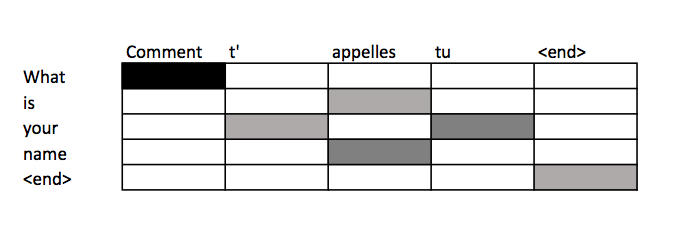
\includegraphics[width=\linewidth]{alignment.png}
	\caption {Example of an alignment table}
	\label{fig:bidir_enc}
\end{marginfigure}

The attention-based model learns to assign significance to different parts of the input for each step of the output.
In the context of translation, attention can be thought of as "alignment." Bahdanau et al. argue that the attention scores $\alpha_{ij}$ at decoding step $i$ signify the words in the source sentence that align with word $i$ in the target. Noting this, we can use attention scores to build an alignment table -- a table mapping words in the source to corresponding words in the target sentence -- based on the learned encoder and decoder from our Seq2Seq NMT system.


\subsection{Performance on long sentences}

\begin{marginfigure}
	\centering
	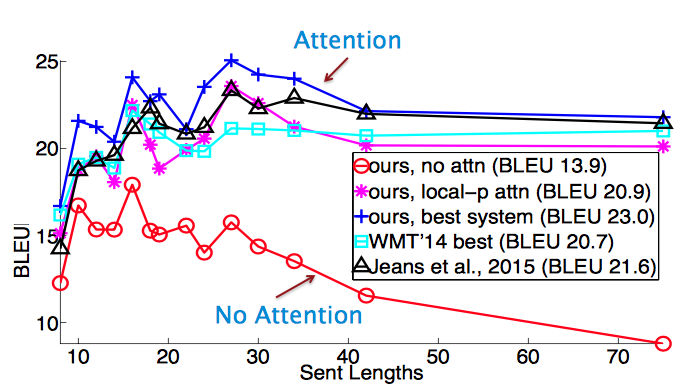
\includegraphics[width=\linewidth]{longsentences.png}
	\caption {Performance on long sentence of different NMT models - image taken from Luong et al.}
	\label{fig:bidir_enc}
\end{marginfigure}

The major advantage of attention-based models is their ability to efficiently translate long sentences. As the size of the input grows, models that do not use attention will miss information and precision if they only use the final representation. Attention is a clever way to fix this issue and experiments indeed confirm the intuition.


\section{Other Models}

\subsection{Huong et al. NMT model}

We present a variant of this first model, with two different mechanisms of attention, from Luong et al.\footnote{\textit{Effective Approaches to Attention-based Neural Machine Translation} by Minh-Thang Luong,  Hieu Pham and Christopher D. Manning}.

\begin{itemize}
\item \textbf{Global attention} We run our vanilla Seq2Seq NMT. We call the hidden states given by the encoder $ h_1, \ldots, h_n $, and the hidden states of the decoder $ \bar{h_1}, \ldots, \bar{h_n}$. Now, for each $ \bar{h_i}$, we compute an attention vector over the encoder hidden. We can use one of the following scoring functions:
%Luong et al. introduced the use of a bilinear form that has become widely adopted.

$$ score(h_i, \bar{h_j}) = \begin{cases}
h_i^T \bar{h_j}\\
h_i^T W \bar{h_j}\\
W [h_i, \bar{h_j}]
\end{cases} \in \mathbb{R} $$

Now that we have a vector of scores, we can compute a context vector in the same way as Bahdanau et al. First, we normalize the scores via a softmax layer to obtain a vector $ \alpha_i = (\alpha_{i, 1}, \ldots , \alpha_{i,n}) $, where $ \alpha_{i,j} = \frac{exp(score(h_j, \bar{h_i}))}{\sum_{k=1}^n exp(score(h_k, \bar{h_i}))} $

$$ c_i = \sum_{j=1}^n \alpha_{i, j} h_j$$

and we can use the context vector and the hidden state to compute a new vector for the $i$-th time step of the decoder

$$ \tilde{h_i} = f([\bar{h_i}, c_i]) $$

The final step is to use the $ \tilde{h_i} $ to make the final prediction of the decoder. To address the issue of coverage, Luong et al. also use an input-feeding approach. The attentional vectors $ \tilde{h_i} $ are fed as input to the decoder, instead of the final prediction. This is similar to Bahdanau et al., who use the context vectors to compute the hidden vectors of the decoder.

\item \textbf{Local attention} the model predicts an aligned position in the input sequence. Then, it computes a context vector using a window centered on this position. The computational cost of this attention step is constant and does not explode with the length of the sentence.
\end{itemize}

The main takeaway of this discussion is to show that they are lots of ways of doing attention.


\subsection{Google's new NMT}

As a brief aside, Google recently made a major breakthrough for NMT via their own translation system \footnote{Johnson et el. 2016, "Google's Multilingual Neural Machine Translation System: Enabling Zero-Shot Translation"}. Rather than maintain a full Seq2Seq model for every pair of language that they support -- each of which would have to be trained individually, which is a tremendous feat in terms of both data and compute time required -- they built a single system that can translate between any two languages. This is a Seq2Seq model that accepts as input a sequence of words \textit{and} a token specifying what language to translate into. The model uses shared parameters to translate into any target language.

\begin{marginfigure}
	\centering
	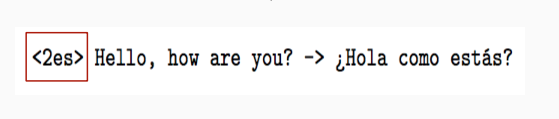
\includegraphics[width=\linewidth]{google_example.png}
	\caption {Example of Google's system}
	\label{fig:bidir_enc}
\end{marginfigure}

The new multilingual model not only improved their translation performance, it also enabled "zero-shot translation," in which we can translate between two languages \textit{for which we have no translation training data}. For instance, if we only had examples of Japanese-English translations and Korean-English translations, Google's team found that the multilingual NMT system trained on this data could actually generate reasonable Japanese-Korean translations. The powerful implication of this finding is that part of the decoding process is not language-specific, and the model is in fact maintaining an internal representation of the input/output sentences independent of the actual languages involved.

\subsection{More advanced papers using attention}

%The previous attention mechanism normalizes the scores over the input sequence. However, we impose no constraint on the coverage of the target sequence. A list of interesting papers that tackle this issue and go beyond the scope of this introduction is


\begin{itemize}
\item \emph{Show, Attend and Tell: Neural Image Caption Generation with Visual Attention} by Kelvin Xu, Jimmy Lei Ba,Ryan Kiros, Kyunghyun Cho, Aaron Courville, Ruslan Salakhutdinov, Richard S. Zemel and Yoshua Bengio. This paper learns words/image alignment.
\item \emph{Modeling Coverage for Neural Machine Translation} by Zhaopeng Tu, Zhengdong Lu, Yang Liu, Xiaohua Liu and Hang Li. Their model uses a coverage vector that takes into account the attention history to help future attention.
\item \emph{Incorporating Structural Alignment Biases into an Attentional Neural Translation Model} by Cohn, Hoang, Vymolova, Yao, Dyer, Haffari. This paper improves the attention by incorporating other traditional linguistic ideas.
\end{itemize}

\section{Sequence model decoders}
Another approach to machine translation comes from statistical machine translation. Consider a model that computes the probability $ \mathbb{P}(\bar{s} | s) $ of a translation $ \bar{s} $ given the original sentence $ s $. We want to pick the translation $ \bar{s}* $ that has the best probability. In other words, we want

$$ \bar{s}* = \operatorname{argmax}_{\bar{s}}(\mathbb{P}(\bar{s} | s )) $$

As the search space can be huge, we need to shrink its size. Here is a list of sequence model decoders (both good ones and bad ones).
\begin{itemize}
\item \textbf{Exhaustive search} : this is the simplest idea. We compute the probability of every possible sequence, and we chose the sequence with the highest probability. However, this technique does not scale \emph{at all} to large outputs as the search space is exponential in the size of the input. Decoding in this case is an NP-complete problem.
\item \textbf{Ancestral sampling} : at time step $ t$, we sample $ x_t $  based on the conditional probability of the word at step $ t$ given the past. In other words,

$$ x_t \sim \mathbb{P}( x_t | x_1, \ldots, x_n) $$

Theoretically, this technique is efficient and asymptotically exact. However, in practice, it can have low performance and high variance.
\item \textbf{Greedy Search} :  At each time step, we pick the most probable token. In other words

$$ x_t = \operatorname{argmax}_{\tilde{x_t}} \mathbb{P}( \tilde{x_t} | x_1, \ldots, x_n) $$

This technique is efficient and natural, however it explores a small part of the search space and if we make a mistake at one time step, the rest of the sentence could be heavily impacted.
\item \textbf{Beam search} : the idea is to maintain $ K $ candidates at each time step.

$$ \mathcal{H}_t = \{ (x_1^1, \ldots, x_t^1), \ldots, (x_1^K, \ldots, x_t^K) \} $$

and compute $ \mathcal{H}_{t+1} $ by expanding $ \mathcal{H}_t $ and keeping the best $ K $ candidates. In other words, we pick the best $ K $ sequence in the following set

$$ \tilde{\mathcal{H}}_{t+1} = \bigcup_{k=1}^K \tilde{\mathcal{H}_{t+1}^k}$$

where

$$ \tilde{\mathcal{H}_{t+1}^k} = \{ (x_1^k, \ldots, x_t^k, v_1), \ldots,  (x_1^k, \ldots, x_t^k, v_{|V|})\}$$

As we increase $ K $, we gain precision and we are asymptotically exact. However, the improvement is not monotonic and we can set a $ K $ that combines reasonable performance and computational efficiency. For this reason, beam search is the most commonly used technique in NMT.
\end{itemize}

\section{Evaluation of Machine Translation Systems}
% from the feb 21 lecture
% no need to cover the LSTM and GRU part that are already covered in past lecture notes
% may just add a reference to it
Now that we know the basics about machine translation systems, we discuss some ways that these models are evaluated. Evaluating the quality of translations is a notoriously tricky and subjective task. In real-life, if you give a paragraph of text to ten different translators, you will get back ten different translations. Translations are imperfect and noisy in practice. They attend to different information and emphasize different meanings. One translation can preserve metaphors and the integrity of long-ranging ideas, while the other can achieve a more faithful reconstruction of syntax and style, attempting a word-to-word translation.  Note that this flexibility is not a burden; it is a testament to the complexity of language and our abilities to decode and interpret meaning, and is a wonderful aspect of our communicative faculty.

At this point, you should note that there is a difference between the objective \textit{loss} function of your model and the \textit{evaluation} methods we are going to discuss. Since loss functions are in essence an evaluation of your model prediction, it can be easy to confuse the two ideas. The evaluation metrics ahead offer a final, summative assessment of your model against some measurement criterion, and no one measurement is superior to all others, though some have clear advantages and majority preference.

Evaluating the quality of machine learning translations has become it own entire research area, with many proposals like TER, METEOR, MaxSim, SEPIA, and RTE-MT. We will focus in these notes on two baseline evaluation methods and BLEU.

\subsection{Human Evaluation}
The first and maybe least surprising method is to have people manually evaluate the correctness, adequacy, and fluency of your system. Like the Turing Test, if you can fool a human into not being able to distinguish a human-made translation with your system translation, your model passes the test for looking like a real-life sentence! The obvious problem with this method is that it is costly and inefficient, though it remains the gold standard for machine translation.

\subsection{Evaluation against another task}
A common way of evaluating machine learning models that output a useful \textit{representation} of some data (a representation being a translation or summary) is that if your predictions are useful for solving some challenging task, then the model must be encoding relevant information in your predictions.
For example, you might think of training your translation predictions on a question-answering task in the translated language. That is, you use the outputs of your system as inputs to a model for some other task (the question-answering). If your second task can perform as well on your predictions as it can on well-formed data in the translated language, it means that your inputs have the relevant information or patterns for meeting the demands of the task.

The issue with this method is that the second task may not be affected by many of the finer points of translation. For example, if you measured the quality of translation on a query-retrieval task (like pulling up the right webpage for a search query), you would find that a translation that preserves the main topic words of the documents but ignores syntax and grammar might still fit the task well. But this itself doesn't mean that the quality of your translations is accurate or faithful. Therefore, determining the quality of the translation model is just shifted to determining the quality of the task itself, which may or may not be a good standard.

\subsection{Bilingual Evaluation Understudy (BLEU)}
In 2002, IBM researchers developed the Bilingual Evaluation Understudy (BLEU) that remains, with its many variants to this day, one of the most respected and reliable methods for machine translation.

The BLEU algorithm evaluates the precision score of a candidate machine translation against a reference human translation. The reference human translation is a assumed to be a \textit{model} example of a translation, and we use n-gram matches as our metric for how similar a candidate translation is to it. Consider a reference sentence A and candidate translation B:

\begin{enumerate}[A]
\item there are many ways to evaluate the quality of a translation, like comparing the number of n-grams between a candidate translation and reference.
\item the quality of a translation is evaluate of n-grams in a reference and with translation.
\end{enumerate}

The BLEU score looks for whether n-grams in the machine translation also appear in the reference translation. Color-coded below are some examples of different size n-grams that are shared between the reference and candidate translation.

\begin{enumerate}[A]
\item there are many ways to evaluate \color{blue} the quality of a translation\color{black}, like comparing the number \color{red} of n-grams \color{black} between a candidate translation and \color{green} reference\color{black}.

\item \color{blue} the quality of a translation \color{black} is evaluate \color{red} of n-grams \color{black} in a \color{green} reference \color{black} and with translation.
\end{enumerate}

The BLEU algorithm identifies all such matches of n-grams above, including the unigram matches, and evaluates the strength of the match with the \textit{precision} score. The precision score is the fraction of n-grams in the translation that also appear in the reference.

The algorithm also satisfies two other constraints. For each n-gram size, a gram in the reference translation cannot be matched more than once. For example, the unigram "a" appears twice in B but only once in A. This only counts for one match between the sentences. Additionally, we impose a brevity penalty so that very small sentences that would achieve a 1.0 precision (a "perfect" matching) are not considered good translations. For example, the single word "there" would achieve a 1.0 precision match, but it is obviously not a good match.

Let us see how to actually compute the BLEU score. First let $k$ be the maximum n-gram that we want to evaluate our score on. That is, if $k=4$, the BLUE score only counts the number of n-grams with length less than or equal to 4, and ignores larger n-grams. Let
\begin{equation*}
p_n =  \# \text{ matched n-grams / \# n-grams in candidate translation}
\end{equation*}
the precision score for the grams of length $n$. Finally, let $w_n = 1/2^n $ be a geometric weighting for the precision of the $n$'th gram. Our brevity penalty is defined as
\begin{equation*}
\beta = e^{\min(0, 1 - \frac{\text{len}_\text{ref}}{\text{len}_\text{MT}})}
\end{equation*}

where $\text{len}_\text{ref}$ is the length of the reference translation and $\text{len}_\text{MT}$ is the length of the machine translation.

The BLEU score is then defined as

\begin{equation*}
\text{BLEU} = \beta\prod_{i=1}^k p_n^{w_n}
\end{equation*}

The BLEU score has been reported to correlate well with human judgment of good translations, and so remains a benchmark for all evaluation metrics following it. However, it does have many limitations. It only works well on the corpus level because any zeros in precision scores will zero the entire BLEU score. Additionally, this BLEU score as presented suffers for only comparing a candidate translation against a single reference, which is surely a noisy representation of the relevant n-grams that need to be matched. Variants of BLEU have modified the algorithm to compare the candidate with multiple reference examples.
Additionally, BLEU scores may only be a necessary but not sufficient benchmark to pass for a good machine translation system. Many researchers have optimized BLEU scores until they have begun to approach the same BLEU scores between reference translations, but the true quality remains far below human translations.

\section{Dealing with the large output vocabulary}
% from the feb 21 lecture
Despite the success of modern NMT systems, they have a hard time dealing with large vocabulary size. Specifically, these Seq2Seq models predict the next word in the sequence by computing a target probabilistic distribution over the entire vocabulary using \textit{softmax}. It turns out that \textbf{softmax} can be quite expensive to compute with a large vocabulary and its complexity also scales proportionally to the vocabulary size. We will now examine a number of approaches to address this issue.
\subsection{Scaling softmax}
A very natural idea is to ask "can we find more efficient ways to compute the target probabilistic distribution?" The answer is Yes! In fact, we've already learned two methods that can reduce the complexity of "softmax", which we'll present a high-level review below (see details in lecture note 1).
\begin{enumerate}
\item \textbf{Noise Contrastive Estimation}\newline
The idea of NCE is to approximate "softmax" by randomly sampling K words from negative samples. As a result, we are reducing the computational complexity by a factor of $\frac{|V|}{K}$, where $|V|$ is the vocabulary size. This method has been proven sucessful in word2vec. A recent work by Zoph et al.\footnote{Zoph et al. 2016, \textit{Simple, Fast Noise-Contrastive Estimation for Large RNN Vocabularies}} applied this technique to learning LSTM language models and they also introduced a trick by using the same samples per mini-batch to make the training GPU-efficient.

\item \textbf{Hierarchical Softmax} \newline
Morin et al.\footnote{Morin et al. 2005, \textit{Hierarchical Probabilistic Neural Network Language Model}}
introduced a binary tree structure to more efficiently compute "softmax". Each probability in the target distribution is calculated by taking a path down the tree which only takes $O(log|V|)$ steps. Notably, even though Hierarchical Softmax saves computation, it cannot be easily parallelized to run efficiently on GPU. This method is used by Kim et al. \footnote{Kim et al. 2015, \textit{Character-Aware Neural Language Models}} to train character-based language models which will be covered in lecture 13.
\end{enumerate}

One limitation for both methods is that they only save computation during training step (when target word is known). At test time, one still has to compute the probability of all words in the vocabulary in order to make predictions.
\subsection{Reducing vocabulary}
Instead of optimizing "softmax", one can also try to reduce the effective vocabulary size which will speed up both training and test steps. A naive way of doing this is to simply limit the vocabulary size to a small number and replace words outside the vocabulary with a tag <UNK>. Now, both training and test time can be significantly reduced but this is obviously not ideal because we may generate outputs with lots of <UNK>.

Jean et al. \footnote{Jean et al. 2015, \textit{On Using Very
Large Target Vocabulary for Neural Machine Translation}} proposed a method to maintain a constant vocabulary size $|V'|$ by partitioning the training data into subsets with $\tau$ unique target words, where $\tau=|V'|$. One subset can be found by sequentially scanning the original data set until $\tau$ unique target words are detected( Figure \ref{fig:partition}). And this process is iterated over the entire data set to produce all mini-batch subsets. In practice, we can achieve about 10x saving with $|V|=500K$ and $|V'|=30K, 50K$.

\begin{marginfigure}
	\centering
	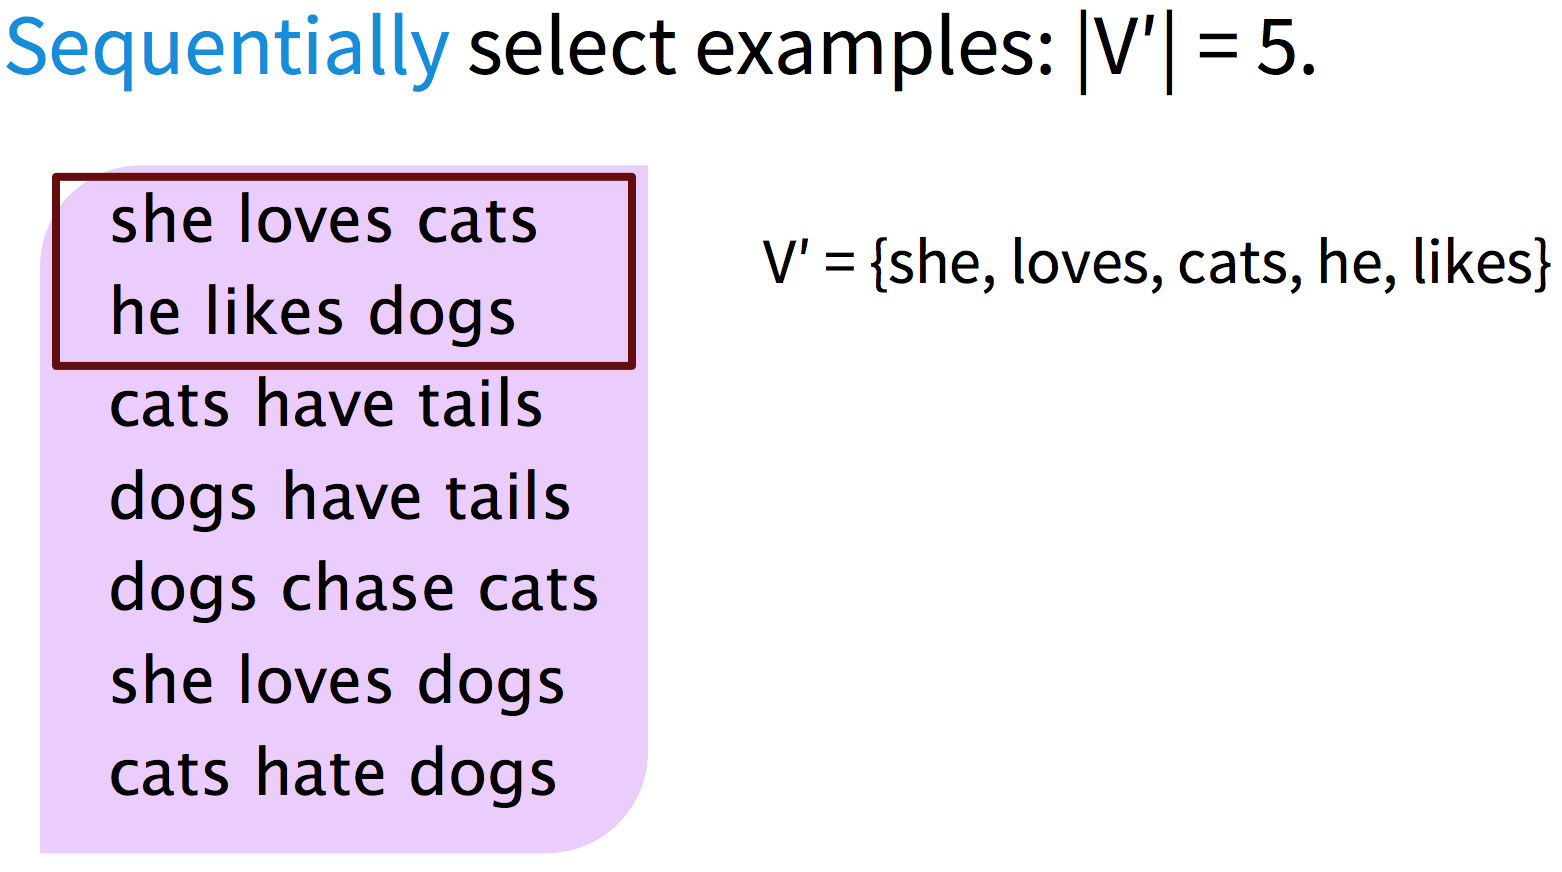
\includegraphics[width=0.9\linewidth]{partition.png}
	\caption {Training data partition}
	\label{fig:partition}
\end{marginfigure}

This concept is very similar to NCE in that for any given word, the output vocabulary contains the target word and $|V'|-1$ negative (noise) samples. However, the main difference is that these negative samples are sampled from a biased distribution $Q$ for each subset V' where
\[
  Q(y_t)=\begin{cases}
               \frac{1}{|V'|}, if y_t \in |V'|\\
               0, otherwise\\
            \end{cases}
\]

At test time, one can similarly predict target word out of a selected subset, called \textit{candidate list}, of the entire vocabulary. The challenge is that the correct target word is unknown and we have to "guess" what the target word might be. In the paper, the authors proposed to construct a candidate list for each source sentence using K most frequent words (based on unigram probability) and K' likely target words for each source word in the sentence. In Figure \ref{fig:candidate}), an example is shown with $K'=3$ and the candidate list consists of all the words in purple boxes. In practice, one can choose the following values: $K =15k,30k,50k$ and $K' = 10, 20$.

\begin{marginfigure}
	\centering
	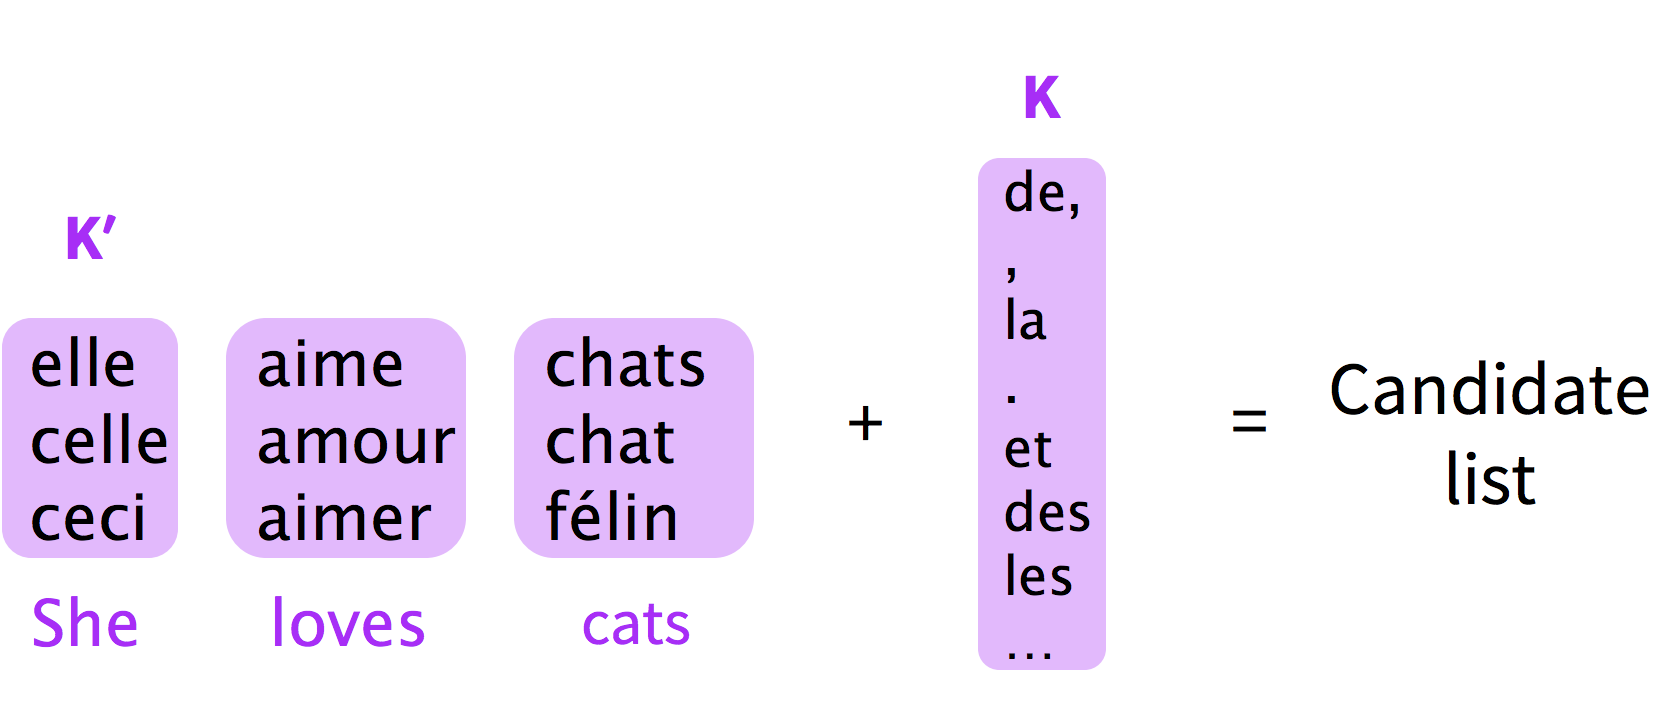
\includegraphics[width=0.9\linewidth]{candidate_list.png}
	\caption {Candidate list}
	\label{fig:candidate}
\end{marginfigure}

\subsection{Handling unknown words}
When NMT systems use the techniques mentioned above to reduce effective vocabulary size, inevitably, certain words will get mapped to <UNK>. For instance, this could happen when the predicted word, usually rare word, is out of the candidate list or when we encounter unseen words at test time. We need new mechanisms to address the rare and unknown word problems.

\begin{marginfigure}
	\centering
	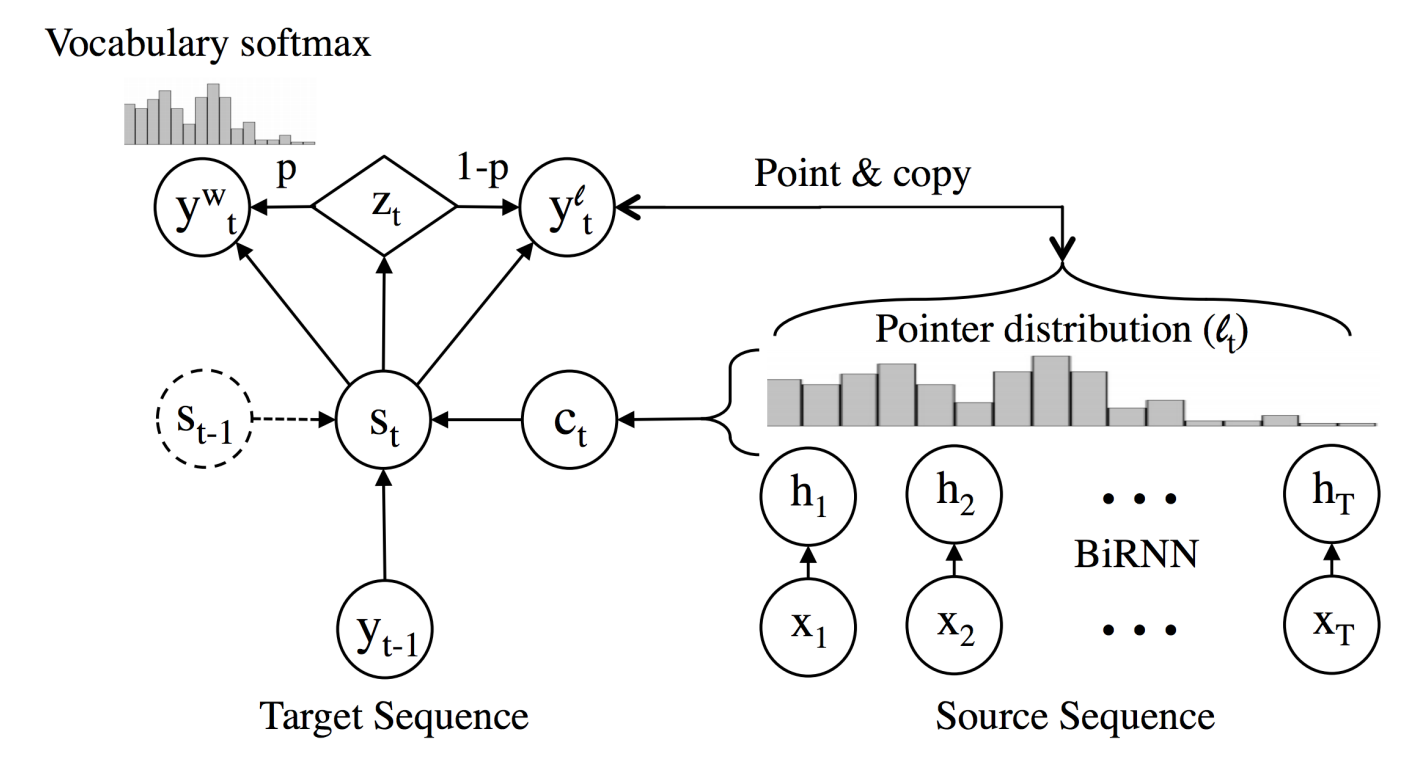
\includegraphics[width=0.9\linewidth]{pointer.png}
	\caption {Pointer network Architecture}
	\label{fig:pointer}
\end{marginfigure}
One idea introduced by Gulcehre et al.\footnote{Gulcehre et al. 2016, \textit{Pointing the Unknown Words}}
to deal with these problems is to learn to "copy" from source text. The model (Figure \ref{fig:pointer}) applies attention distribution $l_t$ to decide \textit{where} to point in the source text and uses the decoder hidden state $S_t$ to predict a binary variable $Z_t$ which decides \textit{when} to copy from source text. The final prediction is either the word $y_t^w$ chosen by softmax over candidate list, as in previous methods, or $y_t^l$ copied from source text depending on the value of $Z_t$.
They showed that this method improves performance in tasks like machine translation and text summarization.


As one can imagine, there are of course limitations to this method. It is important to point out a comment from Google's NMT paper\footnote{Wu et al. 2016, \textit{Google's Neural Machine Translation System: Bridging the Gap
between Human and Machine Translation}} on this method, " \textit{this approach is both unreliable
at scale --- the attention mechanism is unstable when
the network is deep --- and copying may not always be
the best strategy for rare words --- sometimes
transliteration is more appropriate}".



\section{Word and character-based models}
% from the feb 21 lecture
As discussed in section 6, "copy" mechanisms are still not sufficient in dealing with rare or unknown words. Another direction to address these problems is to operate at sub-word levels. One trend is to use the same seq2seq architecture but operate on a smaller unit --- word segmentation, character-based models. Another trend is to embrace hybrid architectures for words and characters.

\subsection{Word segmentation}
Sennrich et al. \footnote{Sennrich et al. 2016, \textit{Neural Machine Translation of Rare Words with Subword Units}} proposed a method to enable open-vocabulary translation by representing rare and unknown words as a sequence of subword units.

\begin{marginfigure}
	\centering
	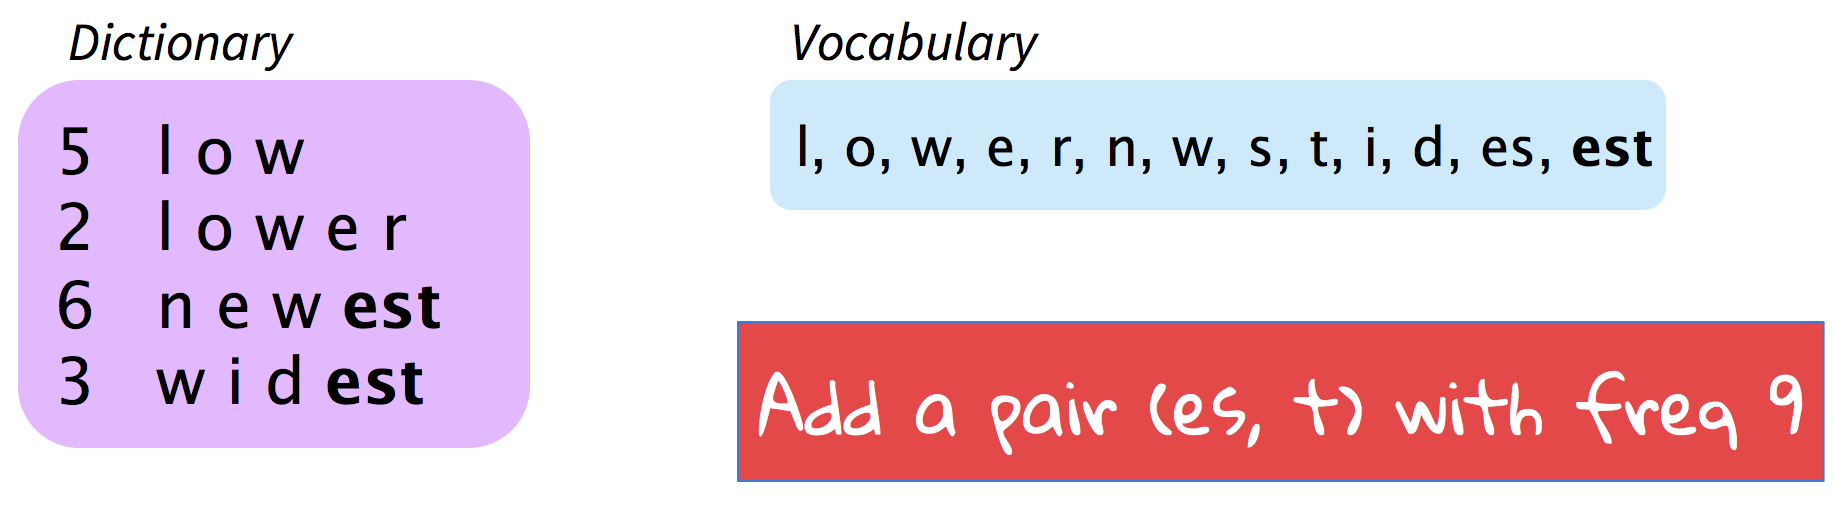
\includegraphics[width=0.9\linewidth]{BPE.png}
	\caption {Byte Pair Encoding}
	\label{fig:BPE}
\end{marginfigure}

This is achieved by adapting a compression algorithm called \textbf{Byte Pair Encoding}. The essential idea is to start with a vocabulary of characters and keep extending the vocabulary with most frequent n-gram pairs in the data set. For instance, in Figure \ref{fig:BPE}, our data set contains 4 words with their frequencies on the left, i.e. "low" appears 5 times. Denote $(p,q,f)$ as a n-gram pair p, q with frequency f. In this figure, we've already selected most frequent n-gram pair (e,s,9) and now we are adding current most frequent n-gram pair (es,t,9). This process is repeated until all n-gram pairs are selected or vocabulary size reaches some threshold.

One can choose to either build separate vocabularies for training and test sets or build one vocabulary jointly. After the vocabulary is built, an NMT system with some seq2seq architecture (the paper used Bahdanau et al. \footnote{Bahdanau et al. 2014, "Neural Machine Translation by Jointly Learning to Align and Translate"}), can be directly trained on these word segments. Notably, this method won top places in WMT 2016.

\subsection{Character-based model}
Ling et al. \footnote{Ling, et al. 2015, "Finding Function in Form: Compositional Character Models for Open Vocabulary Word Representation"} proposed a character-based model to enable open-vocabulary word representation.

For each word $w$ with $m$ characters, instead of storing a word embedding, this model iterates over all characters $c_1,c_2 \ldots c_m$ to look up the character embeddings  $e_1,e_2 \ldots e_m$. These character embeddings are then fed into a biLSTM to get the final hidden states $h_f,h_b$ for forward and backward directions respectively. The final word embedding is computed by an affine transformation of two hidden states:
\[e_w = W_fH_f+W_bH_b + b\]

There are also a family of CNN character-based models which will be covered in lecture 13.

\subsection{Hybrid NMT}
Luong et al. \footnote{Luong et al. 2016, \textit{Achieving Open Vocabulary Neural Machine Translation
with Hybrid Word-Character Models}} proposed a Hybrid Word-Character model to deal with unknown words and achieve open-vocabulary NMT. The system translates mostly at word-level and consults the character components for rare words. On a high level, the character-level recurrent neural networks compute source word representations and recover unknown target words when needed. The twofold advantage of such a hybrid approach is that it is much faster and easier to train than character-based ones; at the same time, it never produces unknown words as in the case of word-based models.

\textbf{Word-based Translation as a Backbone} The core of the hybrid NMT is a deep LSTM encoder-decoder that translates at the word level. We maintain a vocabulary of size $|V|$ per language and use \textit{<unk>} to represent out of vocabulary words.

\begin{marginfigure}
	\centering
	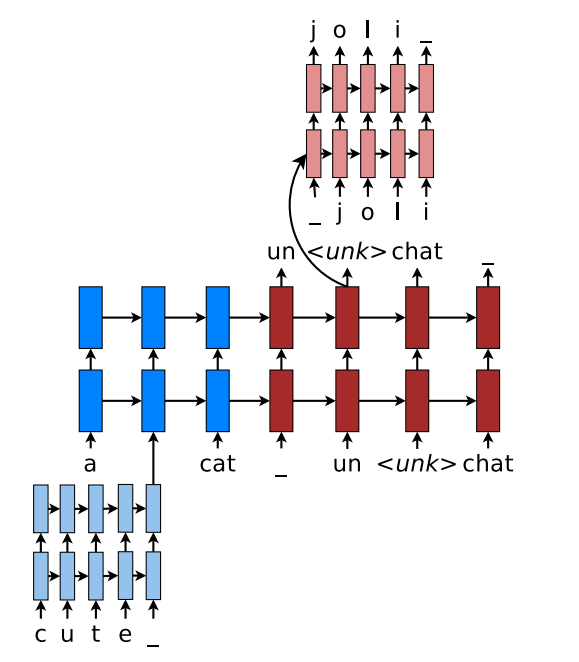
\includegraphics[width=0.9\linewidth]{hybrid.png}
	\caption {Hybrid NMT}
	\label{fig:hybrid}
\end{marginfigure}

\textbf{Source Character-based Representation} In regular word-based NMT, a universal embedding for \textit{<unk>} is used to represent all out-of-vocabulary words. This is problematic because it discards valuable information about the source words. Instead, we learn a deep LSTM model over characters of rare words, and use the final hidden state of the LSTM as the representation for the rare word (Figure \ref{fig:hybrid}).

\textbf{Target Character-level Generation} General word-based NMT allows generation of \textit{<unk>} in the target output. Instead, the goal here is to create a coherent framework that handles an unlimited output vocabulary. The solution is to have a separate deep LSTM that "translates" at the character level given the current word-level state. Note that the current word context is used to initialize the character-level encoder. The system is trained such that whenever the word-level NMT produces an \textit{<unk>}, the character-level decoder is asked to recover the correct surface form of the unknown target word.

%\section{Speech Processing}
% from the feb 23 lecture
% topics yet

\end{document}
